% Options for packages loaded elsewhere
\PassOptionsToPackage{unicode}{hyperref}
\PassOptionsToPackage{hyphens}{url}
\PassOptionsToPackage{dvipsnames,svgnames,x11names}{xcolor}
%
\documentclass[
  man,floatsintext]{apa6}
\usepackage{amsmath,amssymb}
\usepackage{iftex}
\ifPDFTeX
  \usepackage[T1]{fontenc}
  \usepackage[utf8]{inputenc}
  \usepackage{textcomp} % provide euro and other symbols
\else % if luatex or xetex
  \usepackage{unicode-math} % this also loads fontspec
  \defaultfontfeatures{Scale=MatchLowercase}
  \defaultfontfeatures[\rmfamily]{Ligatures=TeX,Scale=1}
\fi
\usepackage{lmodern}
\ifPDFTeX\else
  % xetex/luatex font selection
\fi
% Use upquote if available, for straight quotes in verbatim environments
\IfFileExists{upquote.sty}{\usepackage{upquote}}{}
\IfFileExists{microtype.sty}{% use microtype if available
  \usepackage[]{microtype}
  \UseMicrotypeSet[protrusion]{basicmath} % disable protrusion for tt fonts
}{}
\makeatletter
\@ifundefined{KOMAClassName}{% if non-KOMA class
  \IfFileExists{parskip.sty}{%
    \usepackage{parskip}
  }{% else
    \setlength{\parindent}{0pt}
    \setlength{\parskip}{6pt plus 2pt minus 1pt}}
}{% if KOMA class
  \KOMAoptions{parskip=half}}
\makeatother
\usepackage{xcolor}
\usepackage{color}
\usepackage{fancyvrb}
\newcommand{\VerbBar}{|}
\newcommand{\VERB}{\Verb[commandchars=\\\{\}]}
\DefineVerbatimEnvironment{Highlighting}{Verbatim}{commandchars=\\\{\}}
% Add ',fontsize=\small' for more characters per line
\usepackage{framed}
\definecolor{shadecolor}{RGB}{248,248,248}
\newenvironment{Shaded}{\begin{snugshade}}{\end{snugshade}}
\newcommand{\AlertTok}[1]{\textcolor[rgb]{0.94,0.16,0.16}{#1}}
\newcommand{\AnnotationTok}[1]{\textcolor[rgb]{0.56,0.35,0.01}{\textbf{\textit{#1}}}}
\newcommand{\AttributeTok}[1]{\textcolor[rgb]{0.13,0.29,0.53}{#1}}
\newcommand{\BaseNTok}[1]{\textcolor[rgb]{0.00,0.00,0.81}{#1}}
\newcommand{\BuiltInTok}[1]{#1}
\newcommand{\CharTok}[1]{\textcolor[rgb]{0.31,0.60,0.02}{#1}}
\newcommand{\CommentTok}[1]{\textcolor[rgb]{0.56,0.35,0.01}{\textit{#1}}}
\newcommand{\CommentVarTok}[1]{\textcolor[rgb]{0.56,0.35,0.01}{\textbf{\textit{#1}}}}
\newcommand{\ConstantTok}[1]{\textcolor[rgb]{0.56,0.35,0.01}{#1}}
\newcommand{\ControlFlowTok}[1]{\textcolor[rgb]{0.13,0.29,0.53}{\textbf{#1}}}
\newcommand{\DataTypeTok}[1]{\textcolor[rgb]{0.13,0.29,0.53}{#1}}
\newcommand{\DecValTok}[1]{\textcolor[rgb]{0.00,0.00,0.81}{#1}}
\newcommand{\DocumentationTok}[1]{\textcolor[rgb]{0.56,0.35,0.01}{\textbf{\textit{#1}}}}
\newcommand{\ErrorTok}[1]{\textcolor[rgb]{0.64,0.00,0.00}{\textbf{#1}}}
\newcommand{\ExtensionTok}[1]{#1}
\newcommand{\FloatTok}[1]{\textcolor[rgb]{0.00,0.00,0.81}{#1}}
\newcommand{\FunctionTok}[1]{\textcolor[rgb]{0.13,0.29,0.53}{\textbf{#1}}}
\newcommand{\ImportTok}[1]{#1}
\newcommand{\InformationTok}[1]{\textcolor[rgb]{0.56,0.35,0.01}{\textbf{\textit{#1}}}}
\newcommand{\KeywordTok}[1]{\textcolor[rgb]{0.13,0.29,0.53}{\textbf{#1}}}
\newcommand{\NormalTok}[1]{#1}
\newcommand{\OperatorTok}[1]{\textcolor[rgb]{0.81,0.36,0.00}{\textbf{#1}}}
\newcommand{\OtherTok}[1]{\textcolor[rgb]{0.56,0.35,0.01}{#1}}
\newcommand{\PreprocessorTok}[1]{\textcolor[rgb]{0.56,0.35,0.01}{\textit{#1}}}
\newcommand{\RegionMarkerTok}[1]{#1}
\newcommand{\SpecialCharTok}[1]{\textcolor[rgb]{0.81,0.36,0.00}{\textbf{#1}}}
\newcommand{\SpecialStringTok}[1]{\textcolor[rgb]{0.31,0.60,0.02}{#1}}
\newcommand{\StringTok}[1]{\textcolor[rgb]{0.31,0.60,0.02}{#1}}
\newcommand{\VariableTok}[1]{\textcolor[rgb]{0.00,0.00,0.00}{#1}}
\newcommand{\VerbatimStringTok}[1]{\textcolor[rgb]{0.31,0.60,0.02}{#1}}
\newcommand{\WarningTok}[1]{\textcolor[rgb]{0.56,0.35,0.01}{\textbf{\textit{#1}}}}
\usepackage{graphicx}
\makeatletter
\def\maxwidth{\ifdim\Gin@nat@width>\linewidth\linewidth\else\Gin@nat@width\fi}
\def\maxheight{\ifdim\Gin@nat@height>\textheight\textheight\else\Gin@nat@height\fi}
\makeatother
% Scale images if necessary, so that they will not overflow the page
% margins by default, and it is still possible to overwrite the defaults
% using explicit options in \includegraphics[width, height, ...]{}
\setkeys{Gin}{width=\maxwidth,height=\maxheight,keepaspectratio}
% Set default figure placement to htbp
\makeatletter
\def\fps@figure{htbp}
\makeatother
\setlength{\emergencystretch}{3em} % prevent overfull lines
\providecommand{\tightlist}{%
  \setlength{\itemsep}{0pt}\setlength{\parskip}{0pt}}
\setcounter{secnumdepth}{-\maxdimen} % remove section numbering
% Make \paragraph and \subparagraph free-standing
\ifx\paragraph\undefined\else
  \let\oldparagraph\paragraph
  \renewcommand{\paragraph}[1]{\oldparagraph{#1}\mbox{}}
\fi
\ifx\subparagraph\undefined\else
  \let\oldsubparagraph\subparagraph
  \renewcommand{\subparagraph}[1]{\oldsubparagraph{#1}\mbox{}}
\fi
% definitions for citeproc citations
\NewDocumentCommand\citeproctext{}{}
\NewDocumentCommand\citeproc{mm}{%
  \begingroup\def\citeproctext{#2}\cite{#1}\endgroup}
% avoid brackets around text for \cite:
\makeatletter
 \def\@biblabel#1{}
 \def\@cite#1#2{{#1\if@tempswa , #2\fi}}
\makeatother
\newlength{\cslhangindent}
\setlength{\cslhangindent}{1.5em}
\newlength{\csllabelwidth}
\setlength{\csllabelwidth}{3em}
\newlength{\cslentryspacing}
\setlength{\cslentryspacing}{0em}
\usepackage{enumitem}
\newlist{CSLReferences}{itemize}{1}
\setlist[CSLReferences]{label={},
  leftmargin=\cslhangindent,
  itemindent=-1\cslhangindent,
  parsep=\parskip,
  itemsep=\cslentryspacing}
\usepackage{calc}
\newcommand{\CSLBlock}[1]{#1\hfill\break}
\newcommand{\CSLLeftMargin}[1]{\parbox[t]{\csllabelwidth}{#1}}
\newcommand{\CSLRightInline}[1]{\parbox[t]{\linewidth - \csllabelwidth}{#1}\break}
\newcommand{\CSLIndent}[1]{\hspace{\cslhangindent}#1}
\ifLuaTeX
\usepackage[bidi=basic]{babel}
\else
\usepackage[bidi=default]{babel}
\fi
\babelprovide[main,import]{english}
% get rid of language-specific shorthands (see #6817):
\let\LanguageShortHands\languageshorthands
\def\languageshorthands#1{}
% Manuscript styling
\usepackage{upgreek}
\captionsetup{font=singlespacing,justification=justified}

% Table formatting
\usepackage{longtable}
\usepackage{lscape}
% \usepackage[counterclockwise]{rotating}   % Landscape page setup for large tables
\usepackage{multirow}		% Table styling
\usepackage{tabularx}		% Control Column width
\usepackage[flushleft]{threeparttable}	% Allows for three part tables with a specified notes section
\usepackage{threeparttablex}            % Lets threeparttable work with longtable

% Create new environments so endfloat can handle them
% \newenvironment{ltable}
%   {\begin{landscape}\centering\begin{threeparttable}}
%   {\end{threeparttable}\end{landscape}}
\newenvironment{lltable}{\begin{landscape}\centering\begin{ThreePartTable}}{\end{ThreePartTable}\end{landscape}}

% Enables adjusting longtable caption width to table width
% Solution found at http://golatex.de/longtable-mit-caption-so-breit-wie-die-tabelle-t15767.html
\makeatletter
\newcommand\LastLTentrywidth{1em}
\newlength\longtablewidth
\setlength{\longtablewidth}{1in}
\newcommand{\getlongtablewidth}{\begingroup \ifcsname LT@\roman{LT@tables}\endcsname \global\longtablewidth=0pt \renewcommand{\LT@entry}[2]{\global\advance\longtablewidth by ##2\relax\gdef\LastLTentrywidth{##2}}\@nameuse{LT@\roman{LT@tables}} \fi \endgroup}

% \setlength{\parindent}{0.5in}
% \setlength{\parskip}{0pt plus 0pt minus 0pt}

% Overwrite redefinition of paragraph and subparagraph by the default LaTeX template
% See https://github.com/crsh/papaja/issues/292
\makeatletter
\renewcommand{\paragraph}{\@startsection{paragraph}{4}{\parindent}%
  {0\baselineskip \@plus 0.2ex \@minus 0.2ex}%
  {-1em}%
  {\normalfont\normalsize\bfseries\itshape\typesectitle}}

\renewcommand{\subparagraph}[1]{\@startsection{subparagraph}{5}{1em}%
  {0\baselineskip \@plus 0.2ex \@minus 0.2ex}%
  {-\z@\relax}%
  {\normalfont\normalsize\itshape\hspace{\parindent}{#1}\textit{\addperi}}{\relax}}
\makeatother

\makeatletter
\usepackage{etoolbox}
\patchcmd{\maketitle}
  {\section{\normalfont\normalsize\abstractname}}
  {\section*{\normalfont\normalsize\abstractname}}
  {}{\typeout{Failed to patch abstract.}}
\patchcmd{\maketitle}
  {\section{\protect\normalfont{\@title}}}
  {\section*{\protect\normalfont{\@title}}}
  {}{\typeout{Failed to patch title.}}
\makeatother

\usepackage{xpatch}
\makeatletter
\xapptocmd\appendix
  {\xapptocmd\section
    {\addcontentsline{toc}{section}{\appendixname\ifoneappendix\else~\theappendix\fi\\: #1}}
    {}{\InnerPatchFailed}%
  }
{}{\PatchFailed}
\keywords{APA style, knitr, R, R markdown, papaja\newline\indent Word count: 1,753}
\usepackage{lineno}

\linenumbers
\usepackage{csquotes}
\ifLuaTeX
  \usepackage{selnolig}  % disable illegal ligatures
\fi
\IfFileExists{bookmark.sty}{\usepackage{bookmark}}{\usepackage{hyperref}}
\IfFileExists{xurl.sty}{\usepackage{xurl}}{} % add URL line breaks if available
\urlstyle{same}
\hypersetup{
  pdftitle={How to use papaja: An Example Manuscript Including Basic Instructions},
  pdfauthor={Frederik Aust1},
  pdflang={en-EN},
  pdfkeywords={APA style, knitr, R, R markdown, papaja},
  colorlinks=true,
  linkcolor={blue},
  filecolor={Maroon},
  citecolor={Blue},
  urlcolor={Blue},
  pdfcreator={LaTeX via pandoc}}

\title{How to use \texttt{papaja}: An Example Manuscript Including Basic Instructions}
\author{Frederik Aust\textsuperscript{1}}
\date{}


\shorttitle{How to use papaja}

\authornote{

\texttt{papaja} has not yet been submitted to CRAN; a development version is available at \url{https://github.com/crsh/papaja}.

The authors made the following contributions. Frederik Aust: Conceptualization, Project Administration, Software, Supervision, Validation, Writing - Original Draft Preparation, Writing - Review \& Editing.

Correspondence concerning this article should be addressed to Frederik Aust, Department Psychology, University of Cologne, Herbert-Lewin-Str. 2, 50931 Köln, Germany. E-mail: \href{mailto:frederik.aust@uni-koeln.de}{\nolinkurl{frederik.aust@uni-koeln.de}}

}

\affiliation{\vspace{0.5cm}\textsuperscript{1} University of Cologne}

\abstract{%
This manuscript demonstrates how to use R Markdown and papaja to
create an APA conform manuscript. papaja builds on R Markdown, which
uses pandoc to turn Markdown into PDF or Word documents. The conversion
to Word documents currently supports only a limited set of features.
}



\begin{document}
\maketitle

\section{What is papaja?}\label{what-is-papaja}

Reproducible data analysis is an easy to implement and important aspect of the strive towards reproducibility in science.
For \emph{R} users, R Markdown has been suggested as one possible framework for reproducible analyses.
\texttt{papaja} is a R-package in the making including a \href{https://rmarkdown.rstudio.com/}{R Markdown} template that can be used with (or without) \href{https://posit.co/}{RStudio} to produce documents, which conform to the American Psychological Association (APA) manuscript guidelines (6th Edition).
The package uses the \LaTeX document class \href{http://www.ctan.org/pkg/apa6}{apa6} and a .docx-reference file, so you can create PDF documents, or Word documents if you have to.
Moreover, \texttt{papaja} supplies R-functions that facilitate reporting results of your analyses in accordance with APA guidelines.

Markdown is a simple formatting syntax that can be used to author HTML, PDF, and MS Word documents (among others).
In the following I will assume you know how to use R Markdown to conduct and comment your analyses.
If this is not the case, I recommend you familiarize yourself with \href{https://rmarkdown.rstudio.com/}{R Markdown} first.
I use \href{https://posit.co/}{RStudio} to create my documents, but the general process works with any text editor.

\section{How to use papaja}\label{how-to-use-papaja}

Once you have installed \texttt{papaja} and all other \href{https://github.com/crsh/papaja\#requirements}{required software}, you can select the APA template when creating a new R Markdown file through the RStudio menus, see Figure~\ref{fig:menu}.
When you click RStudio's \emph{Knit} button (see Figure~\ref{fig:knit}), \texttt{papaja}, \texttt{bookdown}, \texttt{rmarkdown,} and \texttt{knitr} work together to create an APA conform manuscript that includes both your text and the output of any embedded R code chunks within the manuscript.



\begin{figure}

{\centering 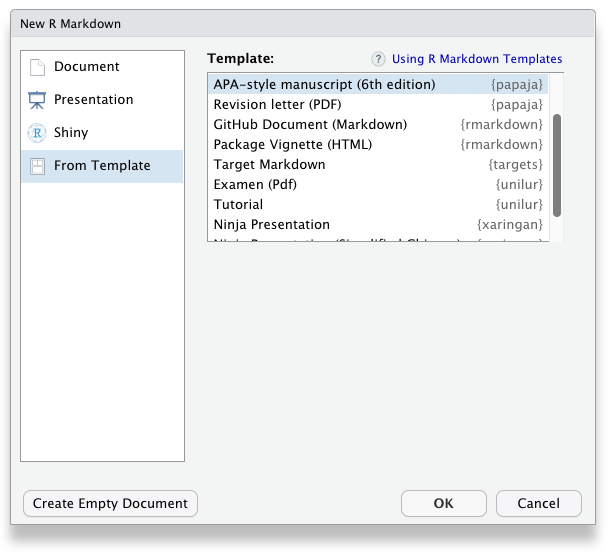
\includegraphics[width=5.69in]{../images/template_selection} 

}

\caption{\texttt{papaja}'s APA6 template is available through the RStudio menus.}\label{fig:menu}
\end{figure}



\begin{figure}

{\centering \includegraphics[width=4.81in]{../images/knitting} 

}

\caption{The Knit button in the RStudio.}\label{fig:knit}
\end{figure}

\subsection{Printing R output}\label{printing-r-output}

Any output from R is included as you usually would using R Markdown.
By default the R code will not be displayed in the final documents.
If you wish to show off your code you need to set \texttt{echo\ =\ TRUE} in the chunk options.
For example, to include summary statistics of your data you could use the following code:

\begin{Shaded}
\begin{Highlighting}[]
\FunctionTok{summary}\NormalTok{(mixed\_data[, }\SpecialCharTok{{-}}\DecValTok{1}\NormalTok{])}
\end{Highlighting}
\end{Shaded}

\begin{verbatim}
##     Subject   Gender Dosage Task   Valence      Recall     
##  A      : 6   F:54   A:36   C:54   Neg:36   Min.   : 4.00  
##  B      : 6   M:54   B:36   F:54   Neu:36   1st Qu.:13.00  
##  C      : 6          C:36          Pos:36   Median :15.00  
##  D      : 6                                 Mean   :15.63  
##  E      : 6                                 3rd Qu.:19.00  
##  F      : 6                                 Max.   :25.00  
##  (Other):72
\end{verbatim}

But, surely, this is not what you want your submission to look like.

\subsubsection{Print tables}\label{print-tables}

For prettier tables, I suggest you try \texttt{apa\_table()}, which builds on \texttt{knitr}'s \texttt{kable()}, and \texttt{apa\_num()}, which can be used to properly round and report numbers.





\begin{Shaded}
\begin{Highlighting}[]
\NormalTok{descriptives }\OtherTok{\textless{}{-}}\NormalTok{ mixed\_data }\SpecialCharTok{\%\textgreater{}\%}
  \FunctionTok{group\_by}\NormalTok{(Dosage) }\SpecialCharTok{\%\textgreater{}\%}
  \FunctionTok{summarize}\NormalTok{(}
    \AttributeTok{Mean =} \FunctionTok{mean}\NormalTok{(Recall)}
\NormalTok{    , }\AttributeTok{Median =} \FunctionTok{median}\NormalTok{(Recall)}
\NormalTok{    , }\AttributeTok{SD =} \FunctionTok{sd}\NormalTok{(Recall)}
\NormalTok{    , }\AttributeTok{Min =} \FunctionTok{min}\NormalTok{(Recall)}
\NormalTok{    , }\AttributeTok{Max =} \FunctionTok{max}\NormalTok{(Recall)}
\NormalTok{  )}
\NormalTok{descriptives[, }\SpecialCharTok{{-}}\DecValTok{1}\NormalTok{] }\OtherTok{\textless{}{-}} \FunctionTok{apa\_num}\NormalTok{(descriptives[, }\SpecialCharTok{{-}}\DecValTok{1}\NormalTok{])}

\FunctionTok{apa\_table}\NormalTok{(}
\NormalTok{  descriptives}
\NormalTok{  , }\AttributeTok{caption =} \StringTok{"(ref:descriptives{-}caption)"}
\NormalTok{  , }\AttributeTok{note =} \StringTok{"(ref:descriptives{-}note)"}
\NormalTok{)}
\end{Highlighting}
\end{Shaded}

\begin{table}[tbp]

\begin{center}
\begin{threeparttable}

\caption{\label{tab:descriptives}Descriptive statistics of correct recall by dosage.}

\begin{tabular}{llllll}
\toprule
Dosage & \multicolumn{1}{c}{Mean} & \multicolumn{1}{c}{Median} & \multicolumn{1}{c}{SD} & \multicolumn{1}{c}{Min} & \multicolumn{1}{c}{Max}\\
\midrule
A & 14.19 & 14.00 & 4.45 & 5 & 25\\
B & 13.50 & 14.00 & 5.15 & 4 & 22\\
C & 19.19 & 19.00 & 3.52 & 13 & 25\\
\bottomrule
\addlinespace
\end{tabular}

\begin{tablenotes}[para]
\normalsize{\textit{Note.} This table was created with \texttt{apa\_table()}.}
\end{tablenotes}

\end{threeparttable}
\end{center}

\end{table}

Of course popular packages like \texttt{xtable}\footnote{When you use \texttt{xtable()}, table captions are \href{http://tex.stackexchange.com/questions/42209/centering-tables-in-document-class-apa6}{set to the left page margin}.} or \texttt{tables} can also be used to create tables when knitting PDF documents.
These packages, however, cannot be used when you want to create Microsoft Word documents because they rely on \LaTeX for typesetting.
\texttt{apa\_table()} creates tables that conform to APA guidelines and are correctly rendered in PDF and Word documents.
But don't get too excited; table formatting is somewhat limited for Word documents due to missing functionality in pandoc (e.g., it is not possible to have cells or headers span across multiple columns).

As required by the APA guidelines, tables are deferred to the final pages of the manuscript when creating a PDF.
Again, this is not the case in Word documents due to limited pandoc functionality.
To place tables and figures in your text instead, set the \texttt{figsintext} parameter in the YAML header to \texttt{yes} or \texttt{true}, as I have done in this document.

The bottom line is, Word documents will be less polished than PDF.
The resulting documents should suffice to enable collaboration with Wordy colleagues and prepare a journal submission with limited manual labor.

\subsubsection{Embed plots}\label{embed-plots}

As usual in R Markdown, you can embed R-generated plots into your document, see Figure~\ref{fig:beeplot}.



\begin{Shaded}
\begin{Highlighting}[]
\FunctionTok{apa\_beeplot}\NormalTok{(}
\NormalTok{  mixed\_data}
\NormalTok{  , }\AttributeTok{id =} \StringTok{"Subject"}
\NormalTok{  , }\AttributeTok{dv =} \StringTok{"Recall"}
\NormalTok{  , }\AttributeTok{factors =} \FunctionTok{c}\NormalTok{(}\StringTok{"Task"}\NormalTok{, }\StringTok{"Valence"}\NormalTok{, }\StringTok{"Dosage"}\NormalTok{)}
\NormalTok{  , }\AttributeTok{dispersion =}\NormalTok{ conf\_int}
\NormalTok{  , }\AttributeTok{ylim =} \FunctionTok{c}\NormalTok{(}\DecValTok{0}\NormalTok{, }\DecValTok{30}\NormalTok{)}
\NormalTok{  , }\AttributeTok{las =} \DecValTok{1}
\NormalTok{  , }\AttributeTok{args\_points =} \FunctionTok{list}\NormalTok{(}\AttributeTok{cex =} \FloatTok{1.5}\NormalTok{)}
\NormalTok{  , }\AttributeTok{args\_arrows =} \FunctionTok{list}\NormalTok{(}\AttributeTok{length =} \FloatTok{0.025}\NormalTok{)}
\NormalTok{)}
\end{Highlighting}
\end{Shaded}

\begin{figure}
\centering
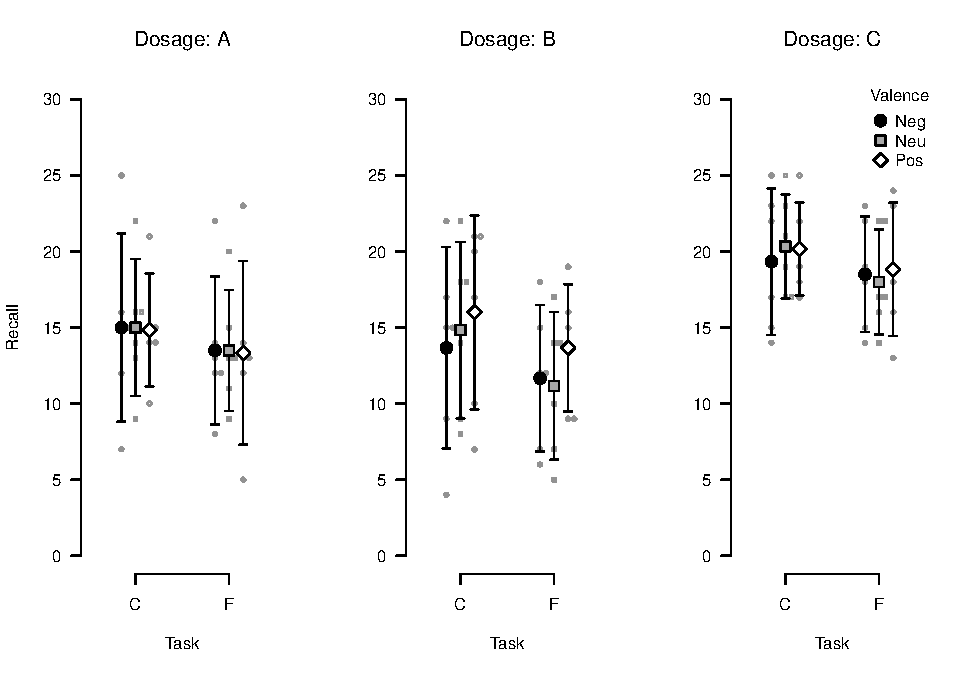
\includegraphics{example_files/figure-latex/beeplot-1.pdf}
\caption{\label{fig:beeplot}Bee plot of the example data set. Small points represent individual observations, large points represent means, and error bars represent 95\% confidence intervals.}
\end{figure}

Again, as required by the APA guidelines, figures are deferred to the final pages of the document unless you set \texttt{figsintext} to \texttt{yes}.

\subsubsection{Referencing figures and tables}\label{referencing-figures-and-tables}

\texttt{papaja} builds on the \texttt{bookdown} package, which provides limited cross-referencing capabilities within documents.
By default you can insert figure and table numbers into the text using \texttt{\textbackslash{}@ref(fig:chunk-name)} for figures or \texttt{\textbackslash{}@ref(tab:chunk-name)} for tables.
Note that for this syntax to work chunk names cannot include \texttt{\_}.
If you need to embed an external image that is not generated by R use the \texttt{knitr::include\_graphics()} function.
See the \href{https://bookdown.org/yihui/bookdown/cross-references.html}{great book on \texttt{bookdown}} for details.
Cross-referencing is currently not available for equations in \texttt{bookdown}.
However, as anywhere in R Markdown documents you can use \LaTeX commands if the functionality is not provided by \texttt{rmarkdown}/\texttt{bookdown} and you don't need to create Word documents.

\subsubsection{Report statistical analyses}\label{report-statistical-analyses}

\texttt{apa\_print()} will help you report the results of your statistical analyses.
The function will format the contents of R objects and produce readily reportable text.

\begin{Shaded}
\begin{Highlighting}[]
\NormalTok{recall\_anova }\OtherTok{\textless{}{-}}\NormalTok{ afex}\SpecialCharTok{::}\FunctionTok{aov\_car}\NormalTok{(}
\NormalTok{  Recall }\SpecialCharTok{\textasciitilde{}}\NormalTok{ (Task }\SpecialCharTok{*}\NormalTok{ Valence }\SpecialCharTok{*}\NormalTok{ Dosage) }\SpecialCharTok{+} \FunctionTok{Error}\NormalTok{(Subject}\SpecialCharTok{/}\NormalTok{(Task }\SpecialCharTok{*}\NormalTok{ Valence)) }\SpecialCharTok{+}\NormalTok{ Dosage}
\NormalTok{  , }\AttributeTok{data =}\NormalTok{ mixed\_data}
\NormalTok{  , }\AttributeTok{type =} \DecValTok{3}
\NormalTok{)}
\NormalTok{recall\_anova\_results }\OtherTok{\textless{}{-}} \FunctionTok{apa\_print}\NormalTok{(recall\_anova, }\AttributeTok{es =} \StringTok{"pes"}\NormalTok{)}
\NormalTok{recall\_anova\_results\_p }\OtherTok{\textless{}{-}} \FunctionTok{apa\_print}\NormalTok{(recall\_anova, }\AttributeTok{es =} \StringTok{"pes"}\NormalTok{, }\AttributeTok{in\_paren =} \ConstantTok{TRUE}\NormalTok{)}
\end{Highlighting}
\end{Shaded}

Now, you can report the results of your analyses like so:

\begin{Shaded}
\begin{Highlighting}[]
\NormalTok{Item }\FunctionTok{valence}\NormalTok{ (}\StringTok{\textasciigrave{}}\AttributeTok{r recall\_anova\_results\_p$full$Valence}\StringTok{\textasciigrave{}}\NormalTok{) and the task}
\NormalTok{affected recall performance, }\StringTok{\textasciigrave{}}\AttributeTok{r recall\_anova\_results$full$Task}\StringTok{\textasciigrave{}}\NormalTok{; the dosage,}
\NormalTok{however, had no effect on recall, }\StringTok{\textasciigrave{}}\AttributeTok{r recall\_anova\_results$full$Dosage}\StringTok{\textasciigrave{}}\NormalTok{.}
\NormalTok{There was no significant interaction.}
\end{Highlighting}
\end{Shaded}

\begin{quote}
Item valence (\(F[1.62, 24.36] = 3.46\), \(\mathit{MSE} = 2.62\), \(p = .056\), \(\hat{\eta}^2_p = .187\)) and the task affected recall performance, \(F(1, 15) = 43.13\), \(\mathit{MSE} = 2.23\), \(p < .001\), \(\hat{\eta}^2_p = .742\);
the dosage, however, had no effect on recall, \(F(2, 15) = 2.97\), \(\mathit{MSE} = 117.17\), \(p = .082\), \(\hat{\eta}^2_p = .283\).
There was no significant interaction.
\end{quote}

What's even more fun, you can easily create a complete ANOVA table using by passing \texttt{recall\_anova\_results\$table} to \texttt{apa\_table()}, see Table~\ref{tab:anova}.





\begin{Shaded}
\begin{Highlighting}[]
\FunctionTok{apa\_table}\NormalTok{(}
\NormalTok{  recall\_anova\_results}\SpecialCharTok{$}\NormalTok{table}
\NormalTok{  , }\AttributeTok{align =} \FunctionTok{c}\NormalTok{(}\StringTok{"l"}\NormalTok{, }\StringTok{"r"}\NormalTok{, }\StringTok{"c"}\NormalTok{, }\StringTok{"r"}\NormalTok{, }\StringTok{"r"}\NormalTok{, }\StringTok{"r"}\NormalTok{)}
\NormalTok{  , }\AttributeTok{caption =} \StringTok{"(ref:anova{-}caption)"}
\NormalTok{  , }\AttributeTok{note =} \StringTok{"(ref:anova{-}note)"}
\NormalTok{)}
\end{Highlighting}
\end{Shaded}

\begin{table}[tbp]

\begin{center}
\begin{threeparttable}

\caption{\label{tab:anova}ANOVA table for the analyis of the example data set.}

\begin{tabular}{lrcrrrl}
\toprule
Effect & \multicolumn{1}{c}{$\hat{\eta}^2_p$} & \multicolumn{1}{c}{$F$} & \multicolumn{1}{c}{$\mathit{df}^{\mathrm{GG}}$} & \multicolumn{1}{c}{$\mathit{df}_{\mathrm{res}}^{\mathrm{GG}}$} & \multicolumn{1}{c}{$\mathit{MSE}$} & \multicolumn{1}{c}{$p$}\\
\midrule
Dosage & .283 & 2.97 & 2 & 15 & 117.17 & .082\\
Task & .742 & 43.13 & 1 & 15 & 2.23 & < .001\\
Valence & .187 & 3.46 & 1.62 & 24.36 & 2.62 & .056\\
Dosage $\times$ Task & .196 & 1.83 & 2 & 15 & 2.23 & .195\\
Dosage $\times$ Valence & .241 & 2.38 & 3.25 & 24.36 & 2.62 & .090\\
Task $\times$ Valence & .091 & 1.50 & 1.35 & 20.20 & 2.67 & .242\\
Dosage $\times$ Task $\times$ Valence & .049 & 0.39 & 2.69 & 20.20 & 2.67 & .743\\
\bottomrule
\addlinespace
\end{tabular}

\begin{tablenotes}[para]
\normalsize{\textit{Note.} This is a table created using \texttt{apa\_print()} and \texttt{apa\_table()}.}
\end{tablenotes}

\end{threeparttable}
\end{center}

\end{table}

\subsection{Citations}\label{citations}

No manuscript is complete without citation.
In order for citations to work, you need to supply a .bib-file to the \texttt{bibliography} parameter in the YAML front matter.
Once this is done, \texttt{{[}e.g.,\ @james\_1890;\ @bem\_2011{]}} produces a regular citation within parentheses (e.g., Bem, 2011; James, 1890).
To cite a source in text simply omit the brackets; for example, write \texttt{@james\_1890} to cite James (1890).
For other options see the \href{https://rmarkdown.rstudio.com/authoring_bibliographies_and_citations.html}{overview of the R Markdown citation syntax}.

The citation style is automatically set to APA style.
If you need to use a different citation style, you can set in the YAML front matter by providing the \texttt{csl} parameter.
See the \href{https://rmarkdown.rstudio.com/authoring_bibliographies_and_citations.html}{R Markdown documentation} and \href{http://citationstyles.org/}{Citation Style Language} for further details.

If you use RStudio, I have created an \href{https://github.com/crsh/citr}{easy-to-use add-in} that facilitates inserting citations into a document.
The relevant references will, of course, be added to the documents reference section automatically.
Moreover, the addin can directly access you Zotero database.

I think it is important to credit the software we use.
A lot of R packages are developed by academics free of charge.
As citations are the currency of science, it's easy to compensate volunteers for their work by citing the R packages we use.
I suspect that, among other things, this is rarely done because it is tedious work.
That's why papaja makes citing R and its packages easy:

\begin{Shaded}
\begin{Highlighting}[]
\FunctionTok{r\_refs}\NormalTok{(}\AttributeTok{file =} \StringTok{"r{-}references.bib"}\NormalTok{)}
\NormalTok{my\_citation }\OtherTok{\textless{}{-}} \FunctionTok{cite\_r}\NormalTok{(}\AttributeTok{file =} \StringTok{"r{-}references.bib"}\NormalTok{)}
\end{Highlighting}
\end{Shaded}

\texttt{r\_refs()} creates a BibTeX file containing citations for R and all currently loaded packages.
\texttt{cite\_r()} takes these citations and turns them into readily reportable text.
\texttt{my\_citation} now contains the following text that you can use in your document: R (Version 4.3.1; R Core Team, 2015) and the R-packages \emph{afex} (Version 1.3.0; Singmann, Bolker, Westfall, \& Aust, 2016), \emph{bindrcpp} (Müller, 2017), \emph{boot} (Version 1.3.28.1; Davison \& Hinkley, 1997), \emph{broom} (Version 1.0.5; Robinson, 2016), \emph{dplyr} (Version 1.1.2; Wickham \& Francois, 2016), \emph{emmeans} (Version 1.8.6; R. Lenth, 2018), \emph{estimability} (Version 1.4.1; R. V. Lenth, 2015), \emph{knitr} (Version 1.43.7; Xie, 2015), \emph{lme4} (Version 1.1.33; Bates, Mächler, Bolker, \& Walker, 2015), \emph{lsmeans} (R. V. Lenth, 2016), \emph{Matrix} (Version 1.5.4.1; Bates \& Maechler, 2016), \emph{MBESS} (Version 4.9.2; Kelley, 2016), \emph{papaja} (Version 0.1.2; Aust \& Barth, 2015), \emph{reshape2} (Version 1.4.4; Wickham, 2007), \emph{rmarkdown} (Version 2.25; Allaire et al., 2016), \emph{testthat} (Version 3.1.10; Wickham, 2011), and \emph{tinylabels} (Version 0.2.3; Barth, 2022)

\subsection{Math}\label{math}

If you need to report formulas, you can use the flexible \LaTeX syntax (it will work in Word documents, too).
Inline math must be enclosed in \texttt{\$} or \texttt{\textbackslash{}(} and \texttt{\textbackslash{})} and the result will look like this: \(d' = z(H) - z(FA)\).
For larger formulas displayed equations are more appropriate; they are enclosed in \texttt{\$\$} or \texttt{\textbackslash{}{[}}and \texttt{\textbackslash{}{]}},

\[
d' = \frac{\mu_{old} - \mu_{new}}{\sqrt{0.5(\sigma^2_{old} + \sigma^2_{new})}}.
\]

\subsection{Document options}\label{document-options}

This text is set as manuscript.
If you want a thesis-like document you can change the \texttt{class} in the YAML front matter from \texttt{man} to \texttt{doc}.
You can also preview a polished journal typesetting by changing the \texttt{class} to \texttt{jou}.
Refer to the \texttt{apa6} document class \href{ftp://ftp.fu-berlin.de/tex/CTAN/macros/latex/contrib/apa6/apa6.pdf}{documentation} for further \texttt{class} options, such as paper size or draft watermarks.

When creating PDF documents, line numbering can be activated by setting the \texttt{linenumbers} argument in the YAML front matter to \texttt{yes}.
Moreover, you can create lists of figure or table captions at the end of the document by setting \texttt{figurelist} or \texttt{tablelist} to \texttt{yes}, respectively.
These option have no effect on Word documents.

\subsection{Last words}\label{last-words}

That's all I have; enjoy writing your manuscript.
If you have any trouble or ideas for improvements, open an \href{https://github.com/crsh/papaja/issues}{issue} on GitHub or open a pull request.
If you want to contribute, take a look at the \href{https://github.com/crsh/papaja/issues}{open issues} if you need inspiration.
Other than that, there are many output objects from analysis methods that we would like \texttt{apa\_print()} to support.
Any new S3/S4-method for this function are always appreciated (e.g., \texttt{factanal}, \texttt{fa}, \texttt{lavaan}, \texttt{lmer}, or \texttt{glmer}).

\section{References}\label{references}

\setlength{\parindent}{-0.5in}
\setlength{\leftskip}{0.5in}

\phantomsection\label{refs}
\setlength{\cslentryspacing}{0em}
\begin{CSLReferences}
\bibitem[\citeproctext]{ref-R-rmarkdown}
Allaire, J., Cheng, J., Xie, Y., McPherson, J., Chang, W., Allen, J., \ldots{} Hyndman, R. (2016). \emph{Rmarkdown: Dynamic documents for r}. Retrieved from \url{https://CRAN.R-project.org/package=rmarkdown}

\bibitem[\citeproctext]{ref-R-papaja}
Aust, F., \& Barth, M. (2015). \emph{Papaja: Create APA manuscripts with RMarkdown}.

\bibitem[\citeproctext]{ref-R-tinylabels}
Barth, M. (2022). \emph{{tinylabels}: Lightweight variable labels}. Retrieved from \url{https://cran.r-project.org/package=tinylabels}

\bibitem[\citeproctext]{ref-R-lme4}
Bates, D., Mächler, M., Bolker, B., \& Walker, S. (2015). Fitting linear mixed-effects models using {lme4}. \emph{Journal of Statistical Software}, \emph{67}(1), 1--48. \url{https://doi.org/10.18637/jss.v067.i01}

\bibitem[\citeproctext]{ref-R-Matrix}
Bates, D., \& Maechler, M. (2016). \emph{Matrix: Sparse and dense matrix classes and methods}. Retrieved from \url{https://CRAN.R-project.org/package=Matrix}

\bibitem[\citeproctext]{ref-bem_2011}
Bem, D. J. (2011). Feeling the future: Experimental evidence for anomalous retroactive influences on cognition and affect. \emph{Journal of Personality and Social Psychology}, \emph{100}(3), 407---425. \url{https://doi.org/10.1037/a0021524}

\bibitem[\citeproctext]{ref-R-boot}
Davison, A. C., \& Hinkley, D. V. (1997). \emph{Bootstrap methods and their applications}. Cambridge: Cambridge University Press. Retrieved from \url{http://statwww.epfl.ch/davison/BMA/}

\bibitem[\citeproctext]{ref-james_1890}
James, W. (1890). \emph{The principles of psychology}. Holt: New York.

\bibitem[\citeproctext]{ref-R-MBESS}
Kelley, K. (2016). \emph{MBESS: The MBESS r package}. Retrieved from \url{https://CRAN.R-project.org/package=MBESS}

\bibitem[\citeproctext]{ref-R-emmeans}
Lenth, R. (2018). \emph{Emmeans: Estimated marginal means, aka least-squares means}. Retrieved from \url{https://CRAN.R-project.org/package=emmeans}

\bibitem[\citeproctext]{ref-R-estimability}
Lenth, R. V. (2015). \emph{Estimability: Tools for assessing estimability of linear predictions}. Retrieved from \url{https://CRAN.R-project.org/package=estimability}

\bibitem[\citeproctext]{ref-R-lsmeans}
Lenth, R. V. (2016). Least-squares means: The {R} package {lsmeans}. \emph{Journal of Statistical Software}, \emph{69}(1), 1--33. \url{https://doi.org/10.18637/jss.v069.i01}

\bibitem[\citeproctext]{ref-R-bindrcpp}
Müller, K. (2017). \emph{Bindrcpp: An 'rcpp' interface to active bindings}. Retrieved from \url{https://CRAN.R-project.org/package=bindrcpp}

\bibitem[\citeproctext]{ref-R-base}
R Core Team. (2015). \emph{R: A language and environment for statistical computing}. Vienna, Austria: R Foundation for Statistical Computing. Retrieved from \url{http://www.R-project.org/}

\bibitem[\citeproctext]{ref-R-broom}
Robinson, D. (2016). \emph{Broom: Convert statistical analysis objects into tidy data frames}. Retrieved from \url{https://CRAN.R-project.org/package=broom}

\bibitem[\citeproctext]{ref-R-afex}
Singmann, H., Bolker, B., Westfall, J., \& Aust, F. (2016). \emph{Afex: Analysis of factorial experiments}. Retrieved from \url{https://CRAN.R-project.org/package=afex}

\bibitem[\citeproctext]{ref-R-reshape2}
Wickham, H. (2007). Reshaping data with the {reshape} package. \emph{Journal of Statistical Software}, \emph{21}(12), 1--20. Retrieved from \url{http://www.jstatsoft.org/v21/i12/}

\bibitem[\citeproctext]{ref-R-testthat}
Wickham, H. (2011). Testthat: Get started with testing. \emph{The R Journal}, \emph{3}, 5--10. Retrieved from \url{http://journal.r-project.org/archive/2011-1/RJournal_2011-1_Wickham.pdf}

\bibitem[\citeproctext]{ref-R-dplyr}
Wickham, H., \& Francois, R. (2016). \emph{Dplyr: A grammar of data manipulation}. Retrieved from \url{https://CRAN.R-project.org/package=dplyr}

\bibitem[\citeproctext]{ref-R-knitr}
Xie, Y. (2015). \emph{Dynamic documents with {R} and knitr} (2nd ed.). Boca Raton, Florida: Chapman; Hall/CRC. Retrieved from \url{http://yihui.org/knitr/}

\end{CSLReferences}


\end{document}
